\documentclass[professionalfont]{beamer}

\usepackage{graphicx}
\usepackage{newtxtext,newtxmath}
\usepackage[backend=bibtex]{biblatex} 
\addbibresource{ref.bib}
\renewcommand*{\bibfont}{\scriptsize}

\usetheme{default}
\usecolortheme{seagull}

\setbeamertemplate{navigation symbols}{}
\setbeamertemplate{itemize item}{\textbullet} 
\setbeamertemplate{bibliography item}[text]
\setbeamertemplate{title page}{
    \begin{center}
        {\textcolor{blue}{\textbf{\fontsize{13}{14}\selectfont
        Improving Language Understanding \\ by Generative Pre-Training}}} \\[1.5cm]
        
        {\fontsize{9}{14}\selectfont Alec Radford, et al \\[0.3cm]
        OpenAI \\[0.3cm]
        2018}
    \end{center}
}
% ------------------ Title ------------------

\begin{document}
\frame{\titlepage}

% ------------------ Slide 1 ------------------

\begin{frame}
\begin{center}
    { \textbf{\textcolor{blue}{ {\fontsize{12}{14}\selectfont Abstract} }} }
\end{center}
\\[0.5cm]

{\fontsize{10}{14}\selectfont 
\begin{itemize}
    \item Large unlabeled text corpora
    
    - It could not be used for training

    \\[0.5cm]

    \item Solution to unlabeled data

    - \textit{Generative pre-training} (Unsupervised)

    - \textit{Discriminative fine-tuning} (Supervised)

    \\[0.5cm]

    \item Experiment with benchmarks

    - We show effectiveness of our approach
\end{itemize}
}

\end{frame}
% ------------------ Slide 2 ------------------

\begin{frame}
\begin{refsection}

\begin{center}
    { \textbf{\textcolor{blue}{ {\fontsize{12}{14}\selectfont Introduction } }} }
\end{center}
\\[0.2cm]

{\fontsize{10}{14}\selectfont 
\begin{itemize}
    \item Need for unsupervised NLP

    - Manually labeling data is time-consuming
    
    \\[0.3cm]
    
    \item Challenge: What type of objectives are effective?

    - Translation\cite{translation}, Predicting next word\cite{predict-next-word}, etc.

    - Each works better for some tasks than others

    \\[0.3cm]

    \item Challenge: How to Transfer the Learned Knowledge?

    - Changing architecture for each task

    - Complicated fine-tuning for each task

    - Adding auxiliary objectives
\end{itemize}
}

\vspace{0.3cm}
\hrule
\printbibliography

\end{refsection}
\end{frame}
% ------------------ Slide 3 ------------------

\begin{frame}
\begin{center}
    { \textbf{\textcolor{blue}{ {\fontsize{12}{14}\selectfont Introduction} }} }
\end{center}
\\[0.5cm]

{\fontsize{10}{14}\selectfont 
\begin{itemize}
    \item We suggest semi-supervised approach
    
    - Unsupervised Pre-training by predicting next word

    - Supervised Fine-tuning for specific task

    \\[0.5cm]

    \item For our architecture, we use the Transformer

    - It outperforms others (RNNs, LSTMs)

    \\[0.5cm]

    \item Experiment - Four types of tasks

    - NLI, QA, Semantic Similarity, Text Classification

    - SOTA on 9 out of 12 benchmarks
\end{itemize}
}

\end{frame}
% ------------------ Slide 4 ------------------

\begin{frame}
\begin{refsection}

\begin{center}
    { \textbf{\textcolor{blue}{ {\fontsize{12}{14}\selectfont Framework} }} }
\end{center}
\\[0.2cm]

\begin{columns}
\column{0.7\textwidth}
    {\fontsize{10}{14}\selectfont 
        \begin{itemize}
            \item Unsupervised pre-training
    
            - We uses decoder-only transformer \cite{transformer-dec}

            - \( L_1(U) = \sum_{i}\log{P(u_i|u_{i-k}, \cdots , u_{i-1};\Theta)} \)

            \\[1.0cm]
            
            \item Supervised fine-tuning
    
            - \( L_2(U) = \sum_{(x,y)}\log{P(y|x^1, \cdots , x^m)} \)

            - \( L_3(U) = L_2(U) + \lambda * L_1(U) \)

            - Auxiliary objective improves generalization
\end{itemize}
}
\column{0.3\textwidth}
    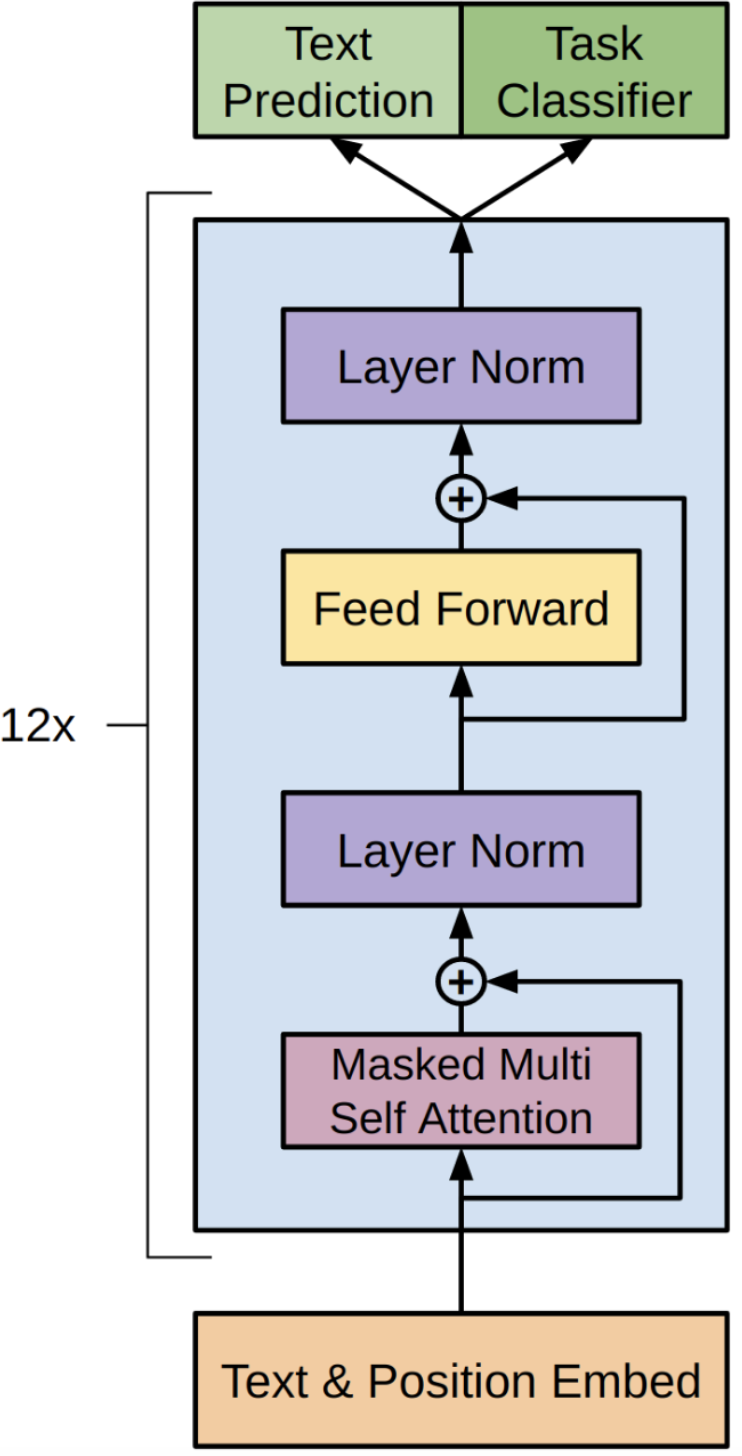
\includegraphics[width=1.0\linewidth]{figure/1-1.png}
\end{columns}

\vspace{0.2cm}
\hrule
\printbibliography

\end{refsection}
\end{frame}
% ------------------ Slide 5 ------------------

\begin{frame}

\begin{center}
    { \textbf{\textcolor{blue}{ {\fontsize{12}{14}\selectfont Framework} }} }
\end{center}
\\[0.2cm]

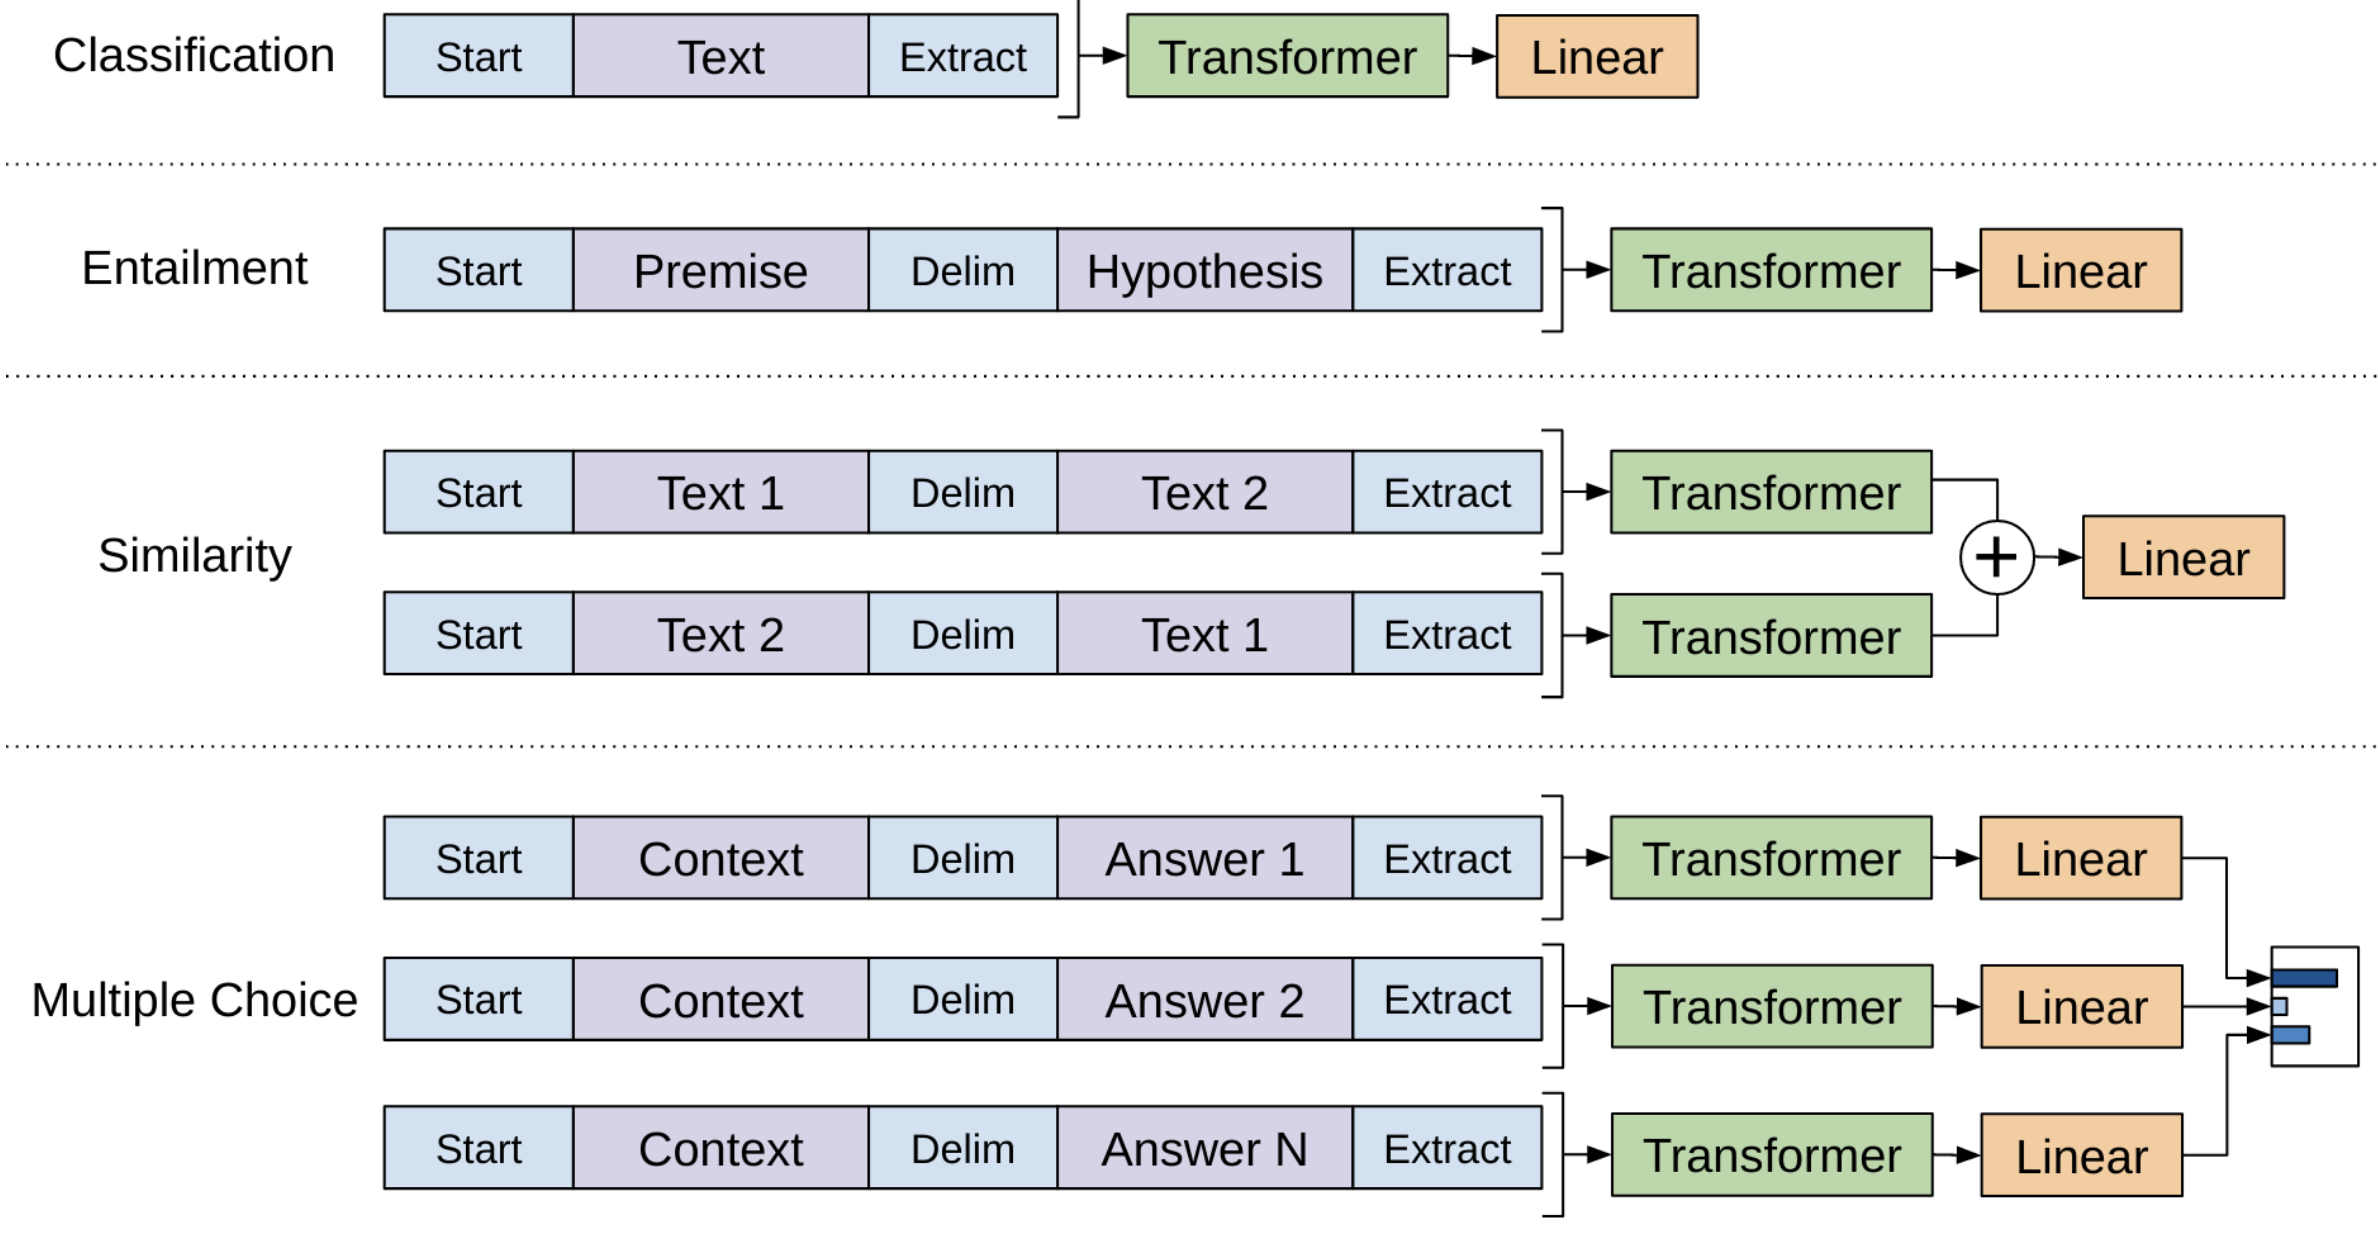
\includegraphics[width=1.0\linewidth]{figure/1-2.png}

\begin{itemize}
    \item Task-specific input transformations
\end{itemize}

\end{frame}
% ------------------ Slide 6 ------------------

\begin{frame}
\begin{refsection}

\begin{center}
    { \textbf{\textcolor{blue}{ {\fontsize{12}{14}\selectfont Experiment} }} }
\end{center}
\\[0.3cm]

\begin{center}
    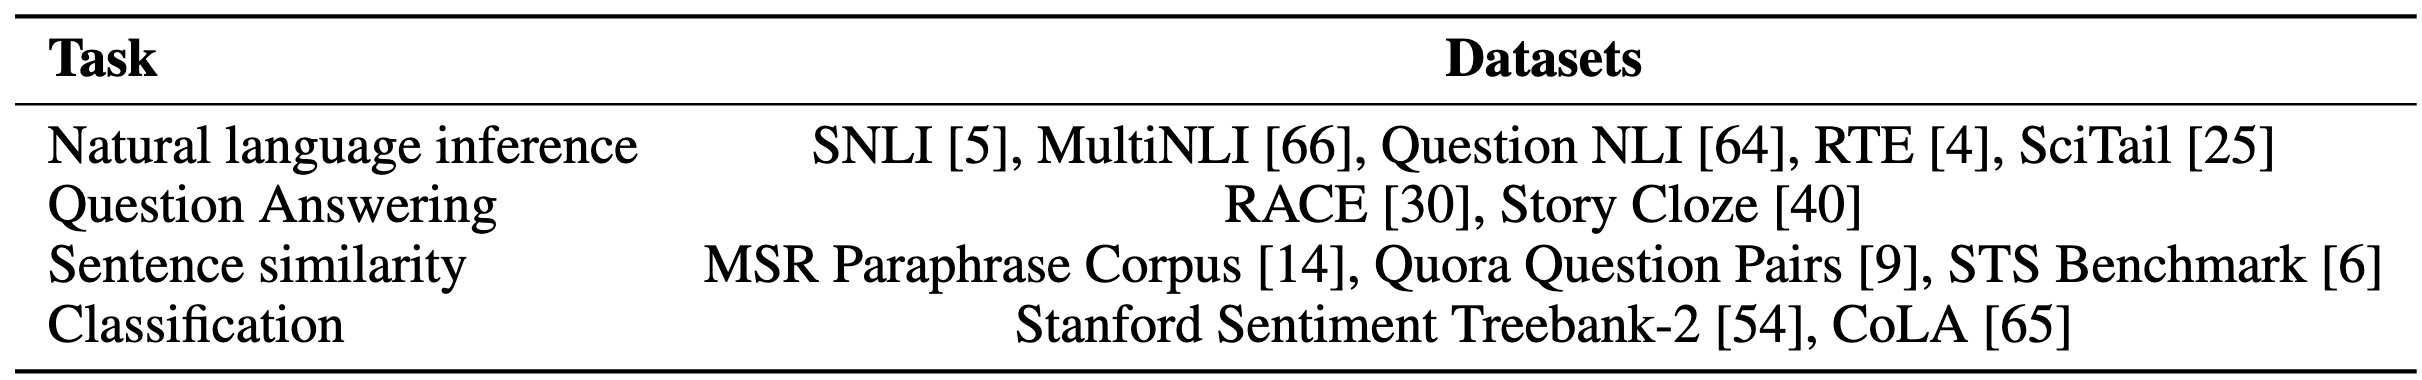
\includegraphics[width=1.0\textwidth]{table/1.png}
\end{center}

{\fontsize{10}{14}\selectfont 
\begin{itemize}
    \item Pre-training

    - BooksCorpus dataset containing 7,000 books \cite{books-corpus}

    \\[0.3cm]

    \item Model specifications

    - Decoder only transformer with 12 layers (unlike BERT)

    - Learned positional embedding instead of sinusoidal

    - Attention - 12 heads and 768 dimension
\end{itemize}
}

\vspace{0.2cm}
\hrule
\printbibliography

\end{refsection}
\end{frame}
% ------------------ Slide 7 ------------------

\begin{frame}
\begin{center}
    { \textbf{\textcolor{blue}{ {\fontsize{12}{14}\selectfont Experiment} }} }
\end{center}
\\[0.3cm]
\begin{center}
    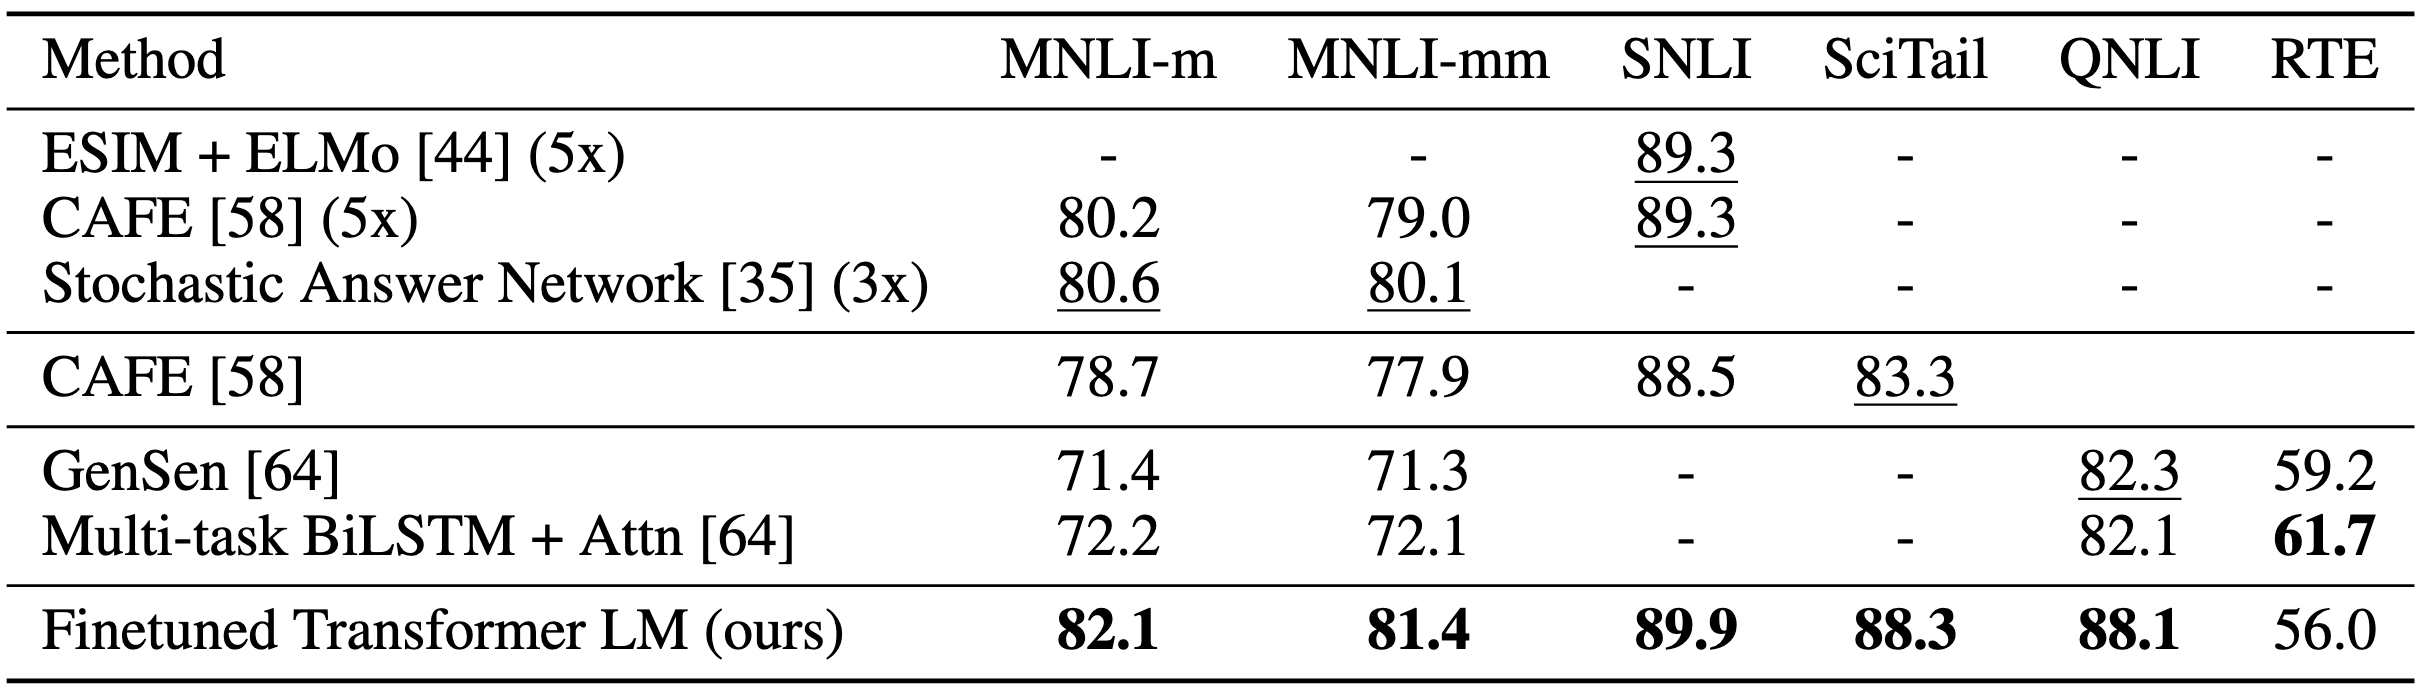
\includegraphics[width=1.0\textwidth]{table/2.png}
\end{center}

{\fontsize{10}{14}\selectfont 
\begin{itemize}
    \item Natural Language Inference
    
    - Given two sentences, determine their relationship

    - Entailment, Contradiction, Neutral

    - GPT outperformed previous SOTA on 4 out of 5

    - RTE is small dataset, making it harder to adapt

\end{itemize}
}

\end{frame}
% ------------------ Slide 8 ------------------

\begin{frame}
\begin{center}
    { \textbf{\textcolor{blue}{ {\fontsize{12}{14}\selectfont Experiment} }} }
\end{center}
\\[0.3cm]
\begin{center}
    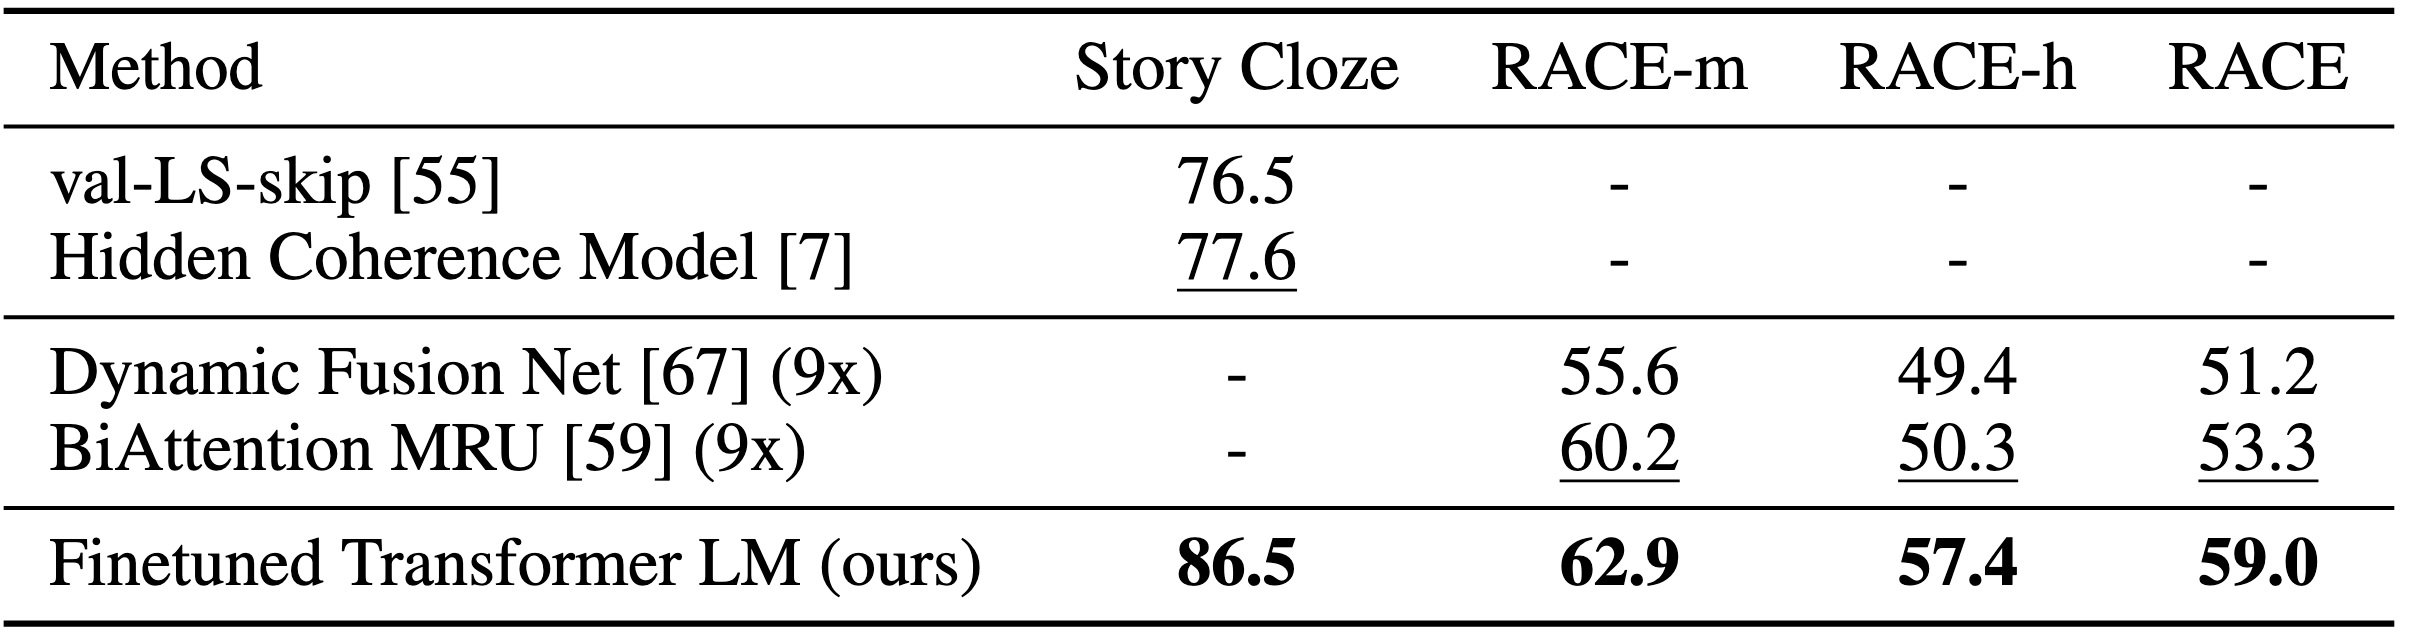
\includegraphics[width=1.0\textwidth]{table/3.png}
\end{center}

{\fontsize{10}{14}\selectfont 
\begin{itemize}
    \item QA and commonsense reasoning

    - Story Cloze: Complete a multi-sentence story

    - RACE: Middle/High School Exams
    
    - GPT outperforms prior SOTA models

    - Transformer allows it to capture long-range dependencies
\end{itemize}
}

\end{frame}
% ------------------ Slide 9 ------------------

\begin{frame}
\begin{center}
    { \textbf{\textcolor{blue}{ {\fontsize{12}{14}\selectfont Experiment} }} }
\end{center}
\\[0.3cm]
\begin{center}
    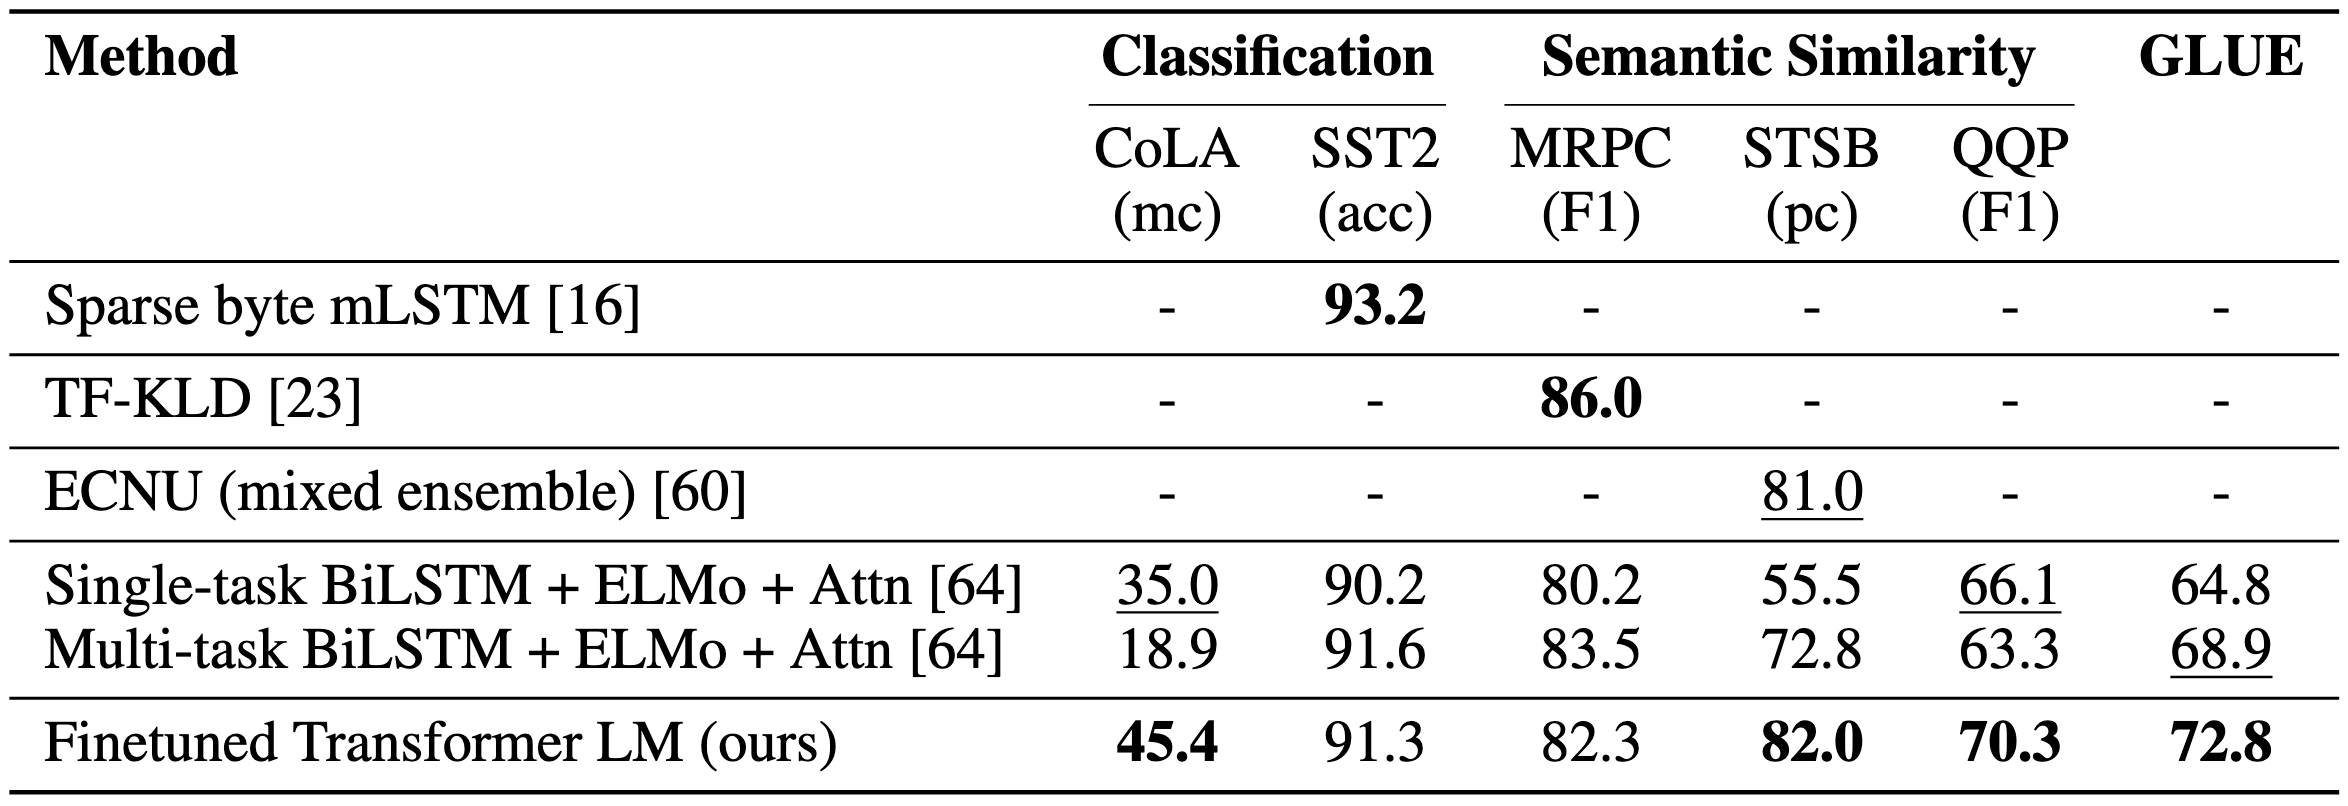
\includegraphics[width=1.0\textwidth]{table/4.png}
\end{center}

{\fontsize{10}{14}\selectfont 
\begin{itemize}
    \item Semantic Similarity

    - Determining if two sentences express the same idea

    - SOTA results on 2 out of 3 datasets
    
    \item Classification

    - CoLA: Is a sentence grammatical?

    - SST: Is a review positive or negative?
\end{itemize}
}

\end{frame}
% ------------------ Slide 10 ------------------

\begin{frame}

\begin{center}
    { \textbf{\textcolor{blue}{ {\fontsize{12}{14}\selectfont Analysis} }} }
\end{center}

\begin{center}
    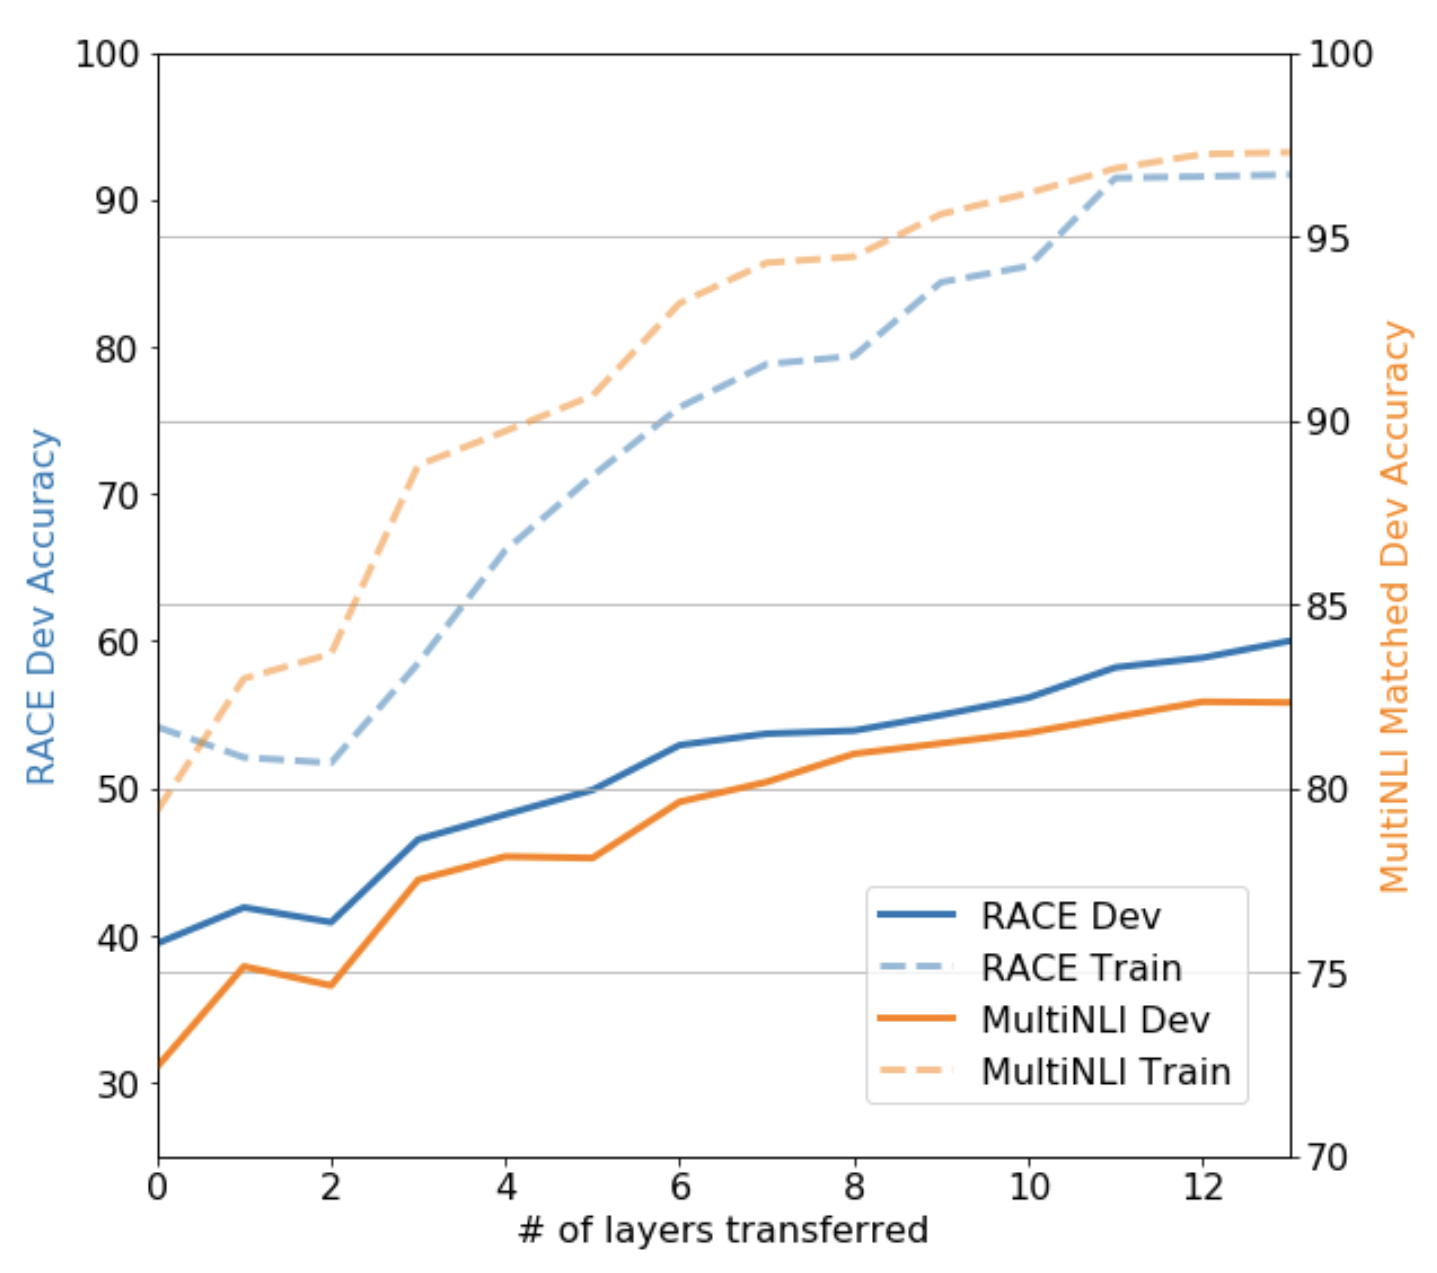
\includegraphics[width=0.6\textwidth]{figure/2-1.png}
\end{center}

{\fontsize{10}{14}\selectfont 
\begin{itemize}
    \item Impact of number of layers transferred

    - Fine-tuning all layers may cause overfitting

    - However, full model transfer leads to best results

\end{itemize}
}

\end{frame}
% ------------------ Slide 11 ------------------

\begin{frame}

\begin{center}
    { \textbf{\textcolor{blue}{ {\fontsize{12}{14}\selectfont Analysis} }} }
\end{center}

\begin{center}
    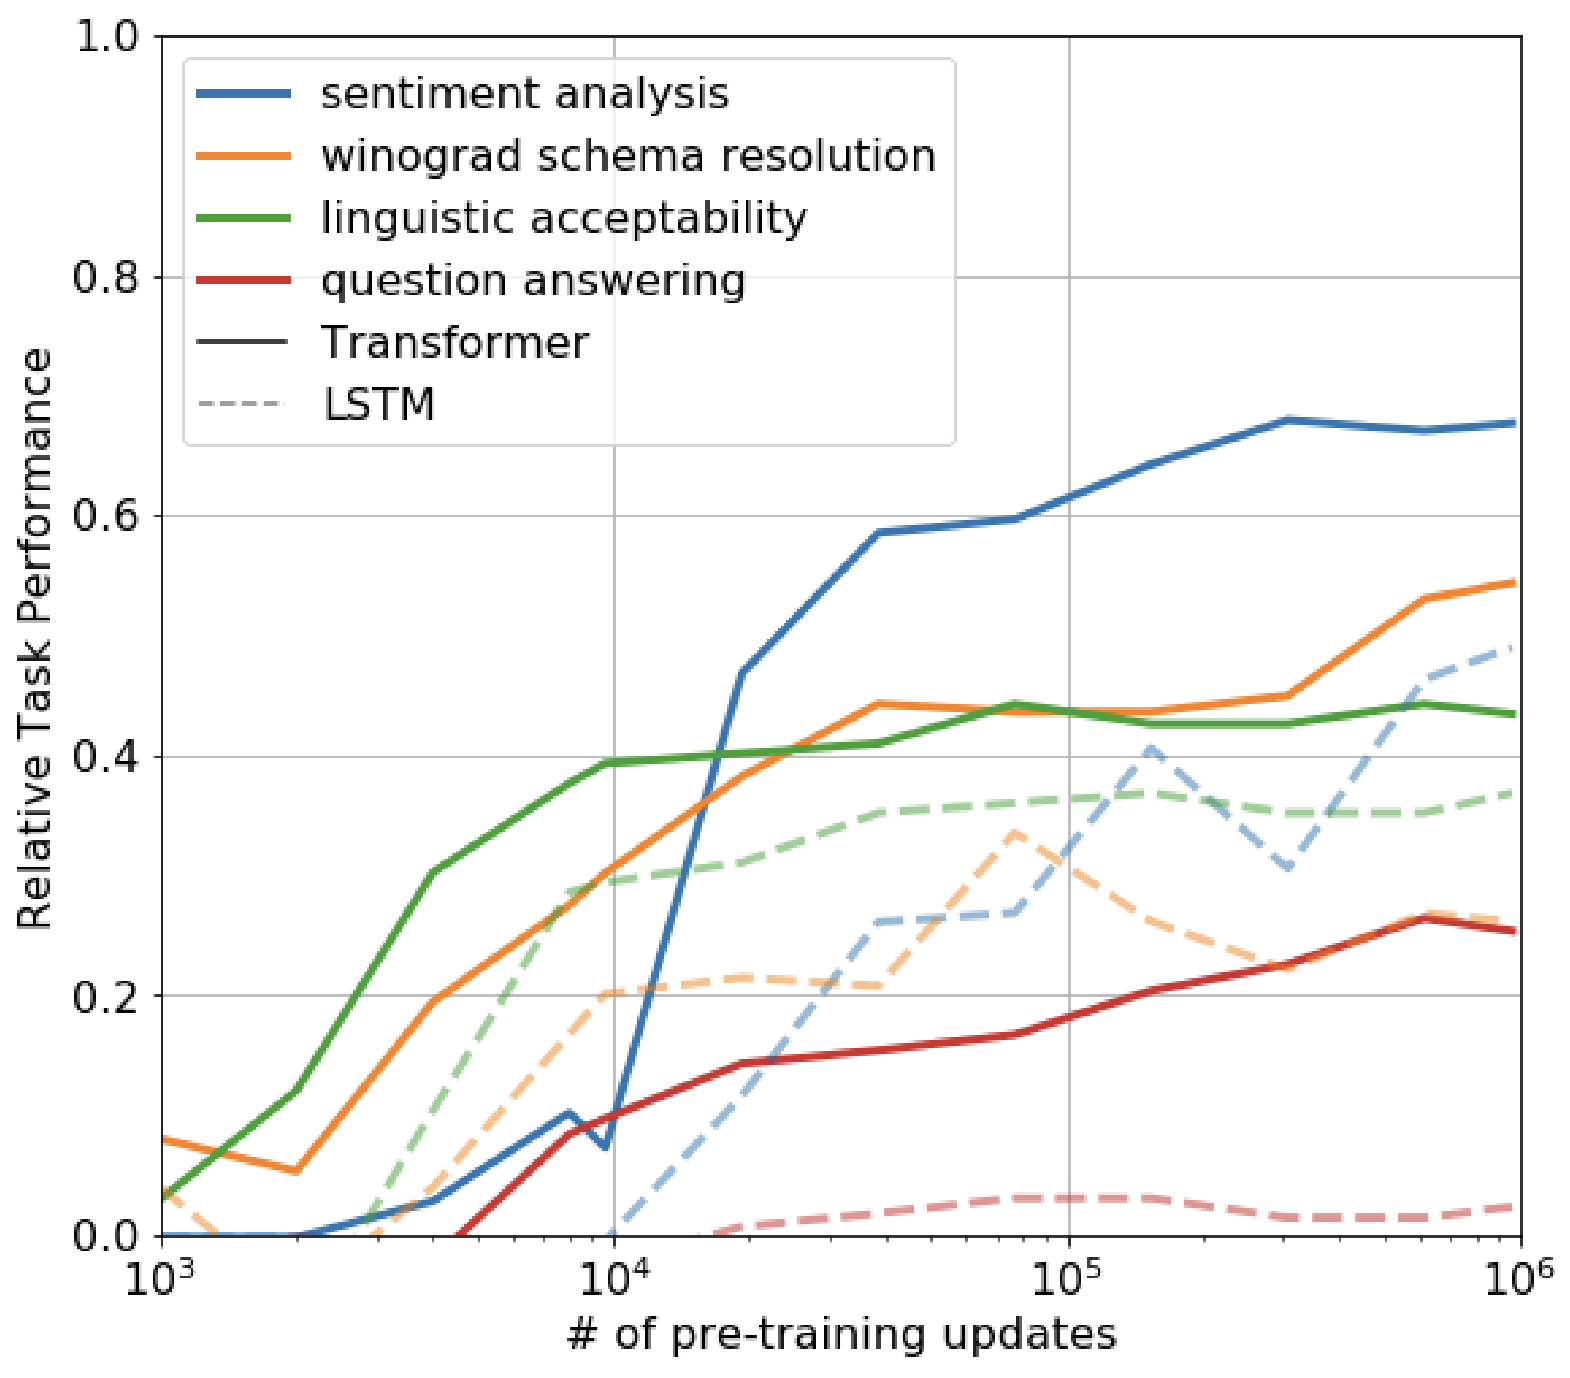
\includegraphics[width=0.6\textwidth]{figure/2-2.png}
\end{center}

{\fontsize{10}{14}\selectfont 
\begin{itemize}
    \item Zero-shot Behaviors (No supervised fine-tuning)
    
    - Performance improves throughout training

    - It means pre-training develops general reasoning abilities

\end{itemize}
}

\end{frame}
% ------------------ Slide 12 ------------------

\begin{frame}

\begin{center}
    { \textbf{\textcolor{blue}{ {\fontsize{12}{14}\selectfont Analysis} }} }
\end{center}
\\[0.3cm]

\begin{center}
    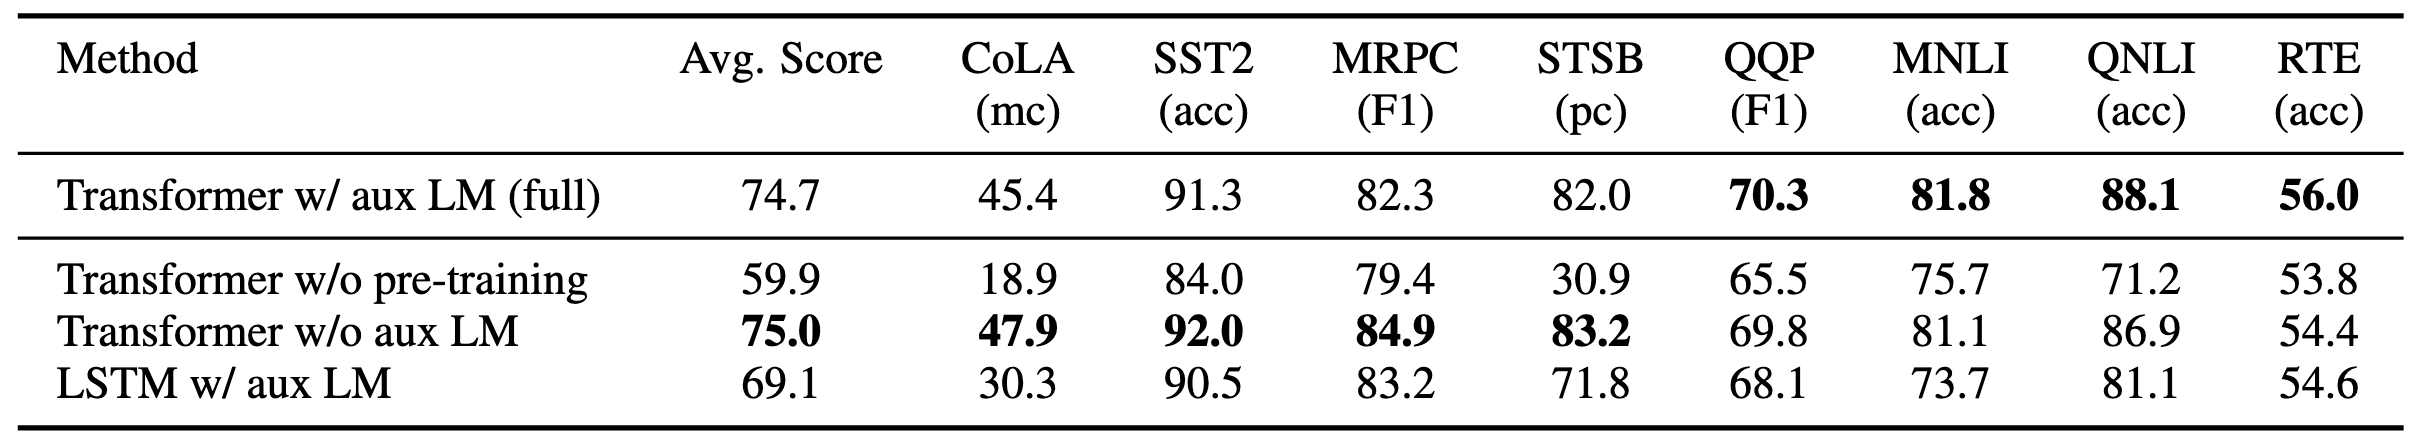
\includegraphics[width=1.0\textwidth]{table/5.png}
\end{center}

{\fontsize{10}{14}\selectfont 
\begin{itemize}
    \item Ablation studies
    
    - Without pre-training, there is massive performance drop

    - Without auxiliary objective, performance drop in larger dataset

    - Using LSTM, model struggles with long-term dependency

\end{itemize}
}

\end{frame}
% ------------------ Slide 13 ------------------

\begin{frame}

\begin{center}
    { \textbf{\textcolor{blue}{ {\fontsize{12}{14}\selectfont Conclusion} }} }
\end{center}
\\[0.3cm]

{\fontsize{10}{14}\selectfont 
\begin{itemize}
    \item Task-agnostic model
    
    - Previous models required task-specific architectures

    - GPT uses one model for multiple NLP tasks

    \\[0.3cm]

    \item Unsupervised learning

    - NLP models relied heavily on supervised learning

    - GPT showed that pre-training on raw text boosts performance

    \\[0.3cm]

    \item Trained on long-form contiguous text

    - Helps capture long-range dependencies in language

    - Provides world knowledge for solving downstream NLP tasks
\end{itemize}
}

\end{frame}
% ------------------ Slide 14 ------------------

\end{document}
